% Nội dung lấy từ slide môn học (ngày 03/11/2026), chỉ giữ các khái niệm mà Chương 3 đến 7 dùng tới
% Hình trong IMAGE/slide/ cắt từ PDF slide ở docs/ bằng script, hình thành phần DSS và 14 đặc trưng vẽ bằng TikZ
\section{Cơ sở lý thuyết}
Mỗi khái niệm trong chương này có mặt vì một chương sau cần tới nó: kho dữ liệu và ETL cho Chương 3, khai phá dữ liệu và cách đo mô hình cho Chương 4 và 5, hệ hỗ trợ ra quyết định cho Chương 6 và 7. Chỗ nào vượt ra ngoài tài liệu môn học thì ghi rõ ngay tại chỗ.

\subsection{Kho dữ liệu}
\subsubsection{Định nghĩa và đặc trưng}
Trong bốn đặc trưng mà Inmon~\cite{inmon2005} gán cho kho dữ liệu, đặc trưng cuối quyết định cách đề tài dựng bảng Snapshot ở Chương 3: kho gắn với thời gian, lưu lịch sử như các ảnh chụp liên tiếp thay vì chỉ giữ trạng thái hiện hành. Ba đặc trưng còn lại là hướng chủ đề (tổ chức theo khách hàng, sản phẩm, doanh số thay vì theo ứng dụng), tích hợp (thống nhất tên và mã hoá từ nhiều nguồn) và không biến động (dữ liệu đã nạp thì chủ yếu để đọc, không sửa liên tục). Bản thân kho dữ liệu (Data Warehouse) là nơi lưu trữ tập trung để phân tích và ra quyết định, gom dữ liệu từ các hệ thống tác nghiệp, làm sạch, chuẩn hoá rồi sắp xếp lại cho phân tích~\cite{inmon2005,kimball2013}.

Hình~\ref{fig:kien_truc_dw} là kiến trúc tổng quát~\cite{elmasri2016}: dữ liệu đi từ các nguồn, qua ETL, vào kho, rồi phục vụ OLAP, DSS và khai phá dữ liệu. Cơ sở dữ liệu tác nghiệp (OLTP) của CompanyX và kho của đề tài khác nhau ở mục đích lẫn cách thiết kế, Bảng~\ref{tab:oltp_olap} đặt hai bên cạnh nhau~\cite{han2011}.

\begin{figure}[!htbp]
\centering
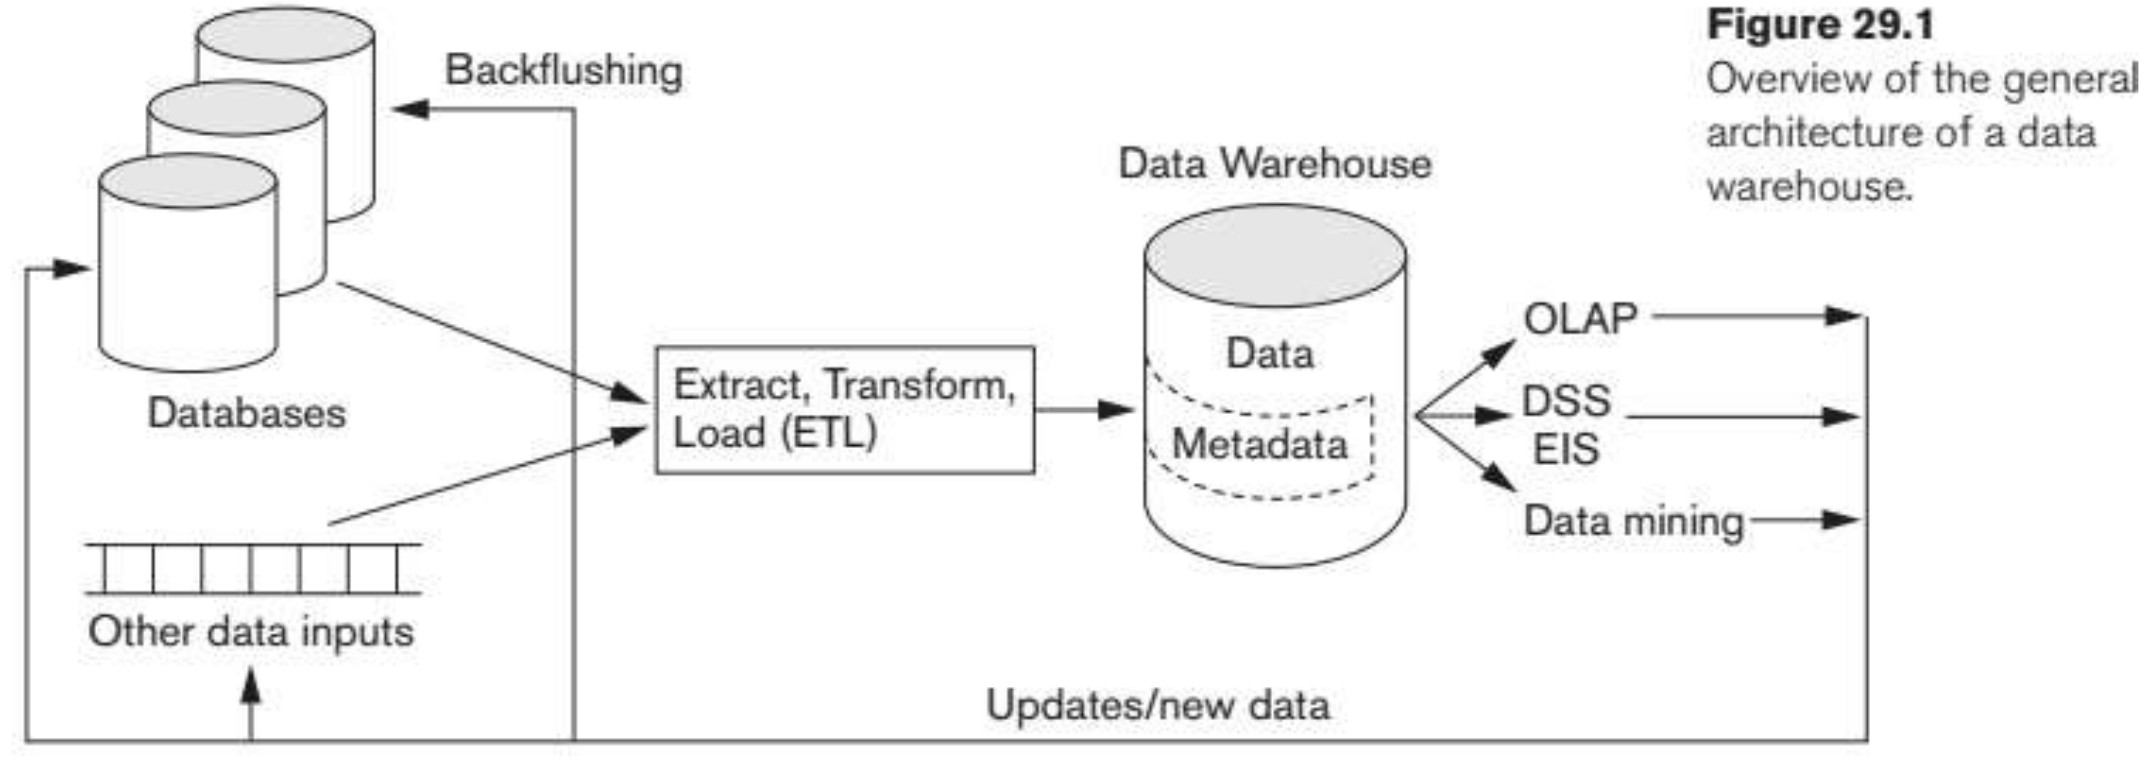
\includegraphics[width=0.9\textwidth]{slide/kien_truc_dw.png}
\caption{Kiến trúc tổng quát của kho dữ liệu}
\label{fig:kien_truc_dw}
\end{figure}

\begin{table}[!htbp]
\centering
\caption{So sánh hệ thống OLTP và OLAP}
\label{tab:oltp_olap}
\begin{tabular}{p{3.2cm}p{5cm}p{5.5cm}}
\toprule
\textbf{Tiêu chí} & \textbf{OLTP} & \textbf{OLAP} \\
\midrule
Định hướng & Giao dịch & Phân tích \\
Người dùng & Nhân viên nhập liệu, quản trị CSDL & Nhà quản lý, chuyên viên phân tích \\
Thiết kế CSDL & Mô hình ER, chuẩn hoá cao & Mô hình sao hoặc bông tuyết, phi chuẩn hoá \\
Dữ liệu & Hiện hành, chi tiết & Lịch sử, tổng hợp, đa chiều \\
Truy cập & Đọc và ghi & Chủ yếu là đọc \\
Đơn vị công việc & Giao dịch ngắn, đơn giản & Truy vấn phức tạp \\
\bottomrule
\end{tabular}
\end{table}

\subsubsection{Mô hình hoá chiều}
Kho ở Chương 3 là một mô hình sao, kiểu thiết kế mà Kimball gọi là mô hình hoá chiều~\cite{kimball2013}. Giữa sao là bảng sự kiện (fact) chứa số đo của nghiệp vụ, ví dụ số tiền bán, cùng khoá ngoại trỏ tới các bảng chiều. Quanh nó là bảng chiều (dimension) chứa thuộc tính mô tả để lọc và nhóm: ngày, sản phẩm, khách hàng. Khi bảng chiều tách nhỏ theo cấp bậc, sao thành bông tuyết (Hình~\ref{fig:sao_bong_tuyet}, vẽ lại theo~\cite{empire}). Kimball thiết kế theo bốn bước: chọn quy trình nghiệp vụ, khai báo độ mịn (một dòng sự kiện thể hiện điều gì), xác định các chiều, xác định các số đo. Thuộc tính của chiều đổi theo thời gian thì xử lý bằng chiều thay đổi chậm (SCD): kiểu 1 ghi đè giá trị cũ, kiểu 2 thêm dòng mới để giữ lịch sử.

\begin{figure}[!htbp]
\centering
% Vẽ lại theo hình trong slide (ảnh cắt từ slide bị chồng hình)
\tikzset{
    chieu/.style={draw, font=\scriptsize, align=center, minimum width=13mm, minimum height=6mm, inner sep=2pt},
    sukien/.style={chieu, fill=gray!15, thick, minimum width=15mm, minimum height=9mm}}
\begin{subfigure}[b]{0.40\textwidth}
    \centering
    \begin{tikzpicture}
        \node[sukien] (fact) {Sales\\Facts};
        \node[chieu, above left=4mm and 3mm of fact] (time) {Time};
        \node[chieu, above right=4mm and 3mm of fact] (cust) {Customer};
        \node[chieu, below left=4mm and 3mm of fact] (prod) {Product};
        \node[chieu, below right=4mm and 3mm of fact] (sell) {Seller};
        \foreach \n in {time,cust,prod,sell} \draw (fact) -- (\n);
    \end{tikzpicture}
    \caption{Mô hình sao}
\end{subfigure}
\hfill
\begin{subfigure}[b]{0.56\textwidth}
    \centering
    \begin{tikzpicture}
        \node[sukien] (fact) {Sales\\Facts};
        \node[chieu, above left=4mm and 3mm of fact] (time) {Time};
        \node[chieu, above right=4mm and 3mm of fact] (cust) {Customer};
        \node[chieu, below left=4mm and 3mm of fact] (prod) {Product};
        \node[chieu, below right=4mm and 3mm of fact] (sell) {Seller};
        \node[chieu, left=3mm of time] (month) {Month};
        \node[chieu, right=3mm of cust] (region) {Region};
        \node[chieu, left=3mm of prod] (cat) {Category};
        \node[chieu, right=3mm of sell] (outlet) {Outlet};
        \foreach \n in {time,cust,prod,sell} \draw (fact) -- (\n);
        \draw (time) -- (month); \draw (cust) -- (region);
        \draw (prod) -- (cat); \draw (sell) -- (outlet);
    \end{tikzpicture}
    \caption{Mô hình bông tuyết}
\end{subfigure}
\caption{Mô hình sao và mô hình bông tuyết}
\label{fig:sao_bong_tuyet}
\end{figure}

\subsubsection{Quy trình ETL và chất lượng dữ liệu}\label{sec:ltetl}
ETL gồm ba bước: trích xuất (Extract) lấy dữ liệu từ nguồn, biến đổi (Transform) làm sạch, đổi định dạng và hợp nhất, nạp (Load) đưa vào kho. Biến thể ELT nạp dữ liệu thô vào kho trước rồi mới biến đổi. Chỗ khó không nằm ở ba động từ đó mà ở tích hợp: các nguồn đặt tên hay mã hoá khác nhau, dữ liệu thiếu, sai hay không nhất quán, nên ETL phải kiểm tra chất lượng trước khi ai đó tin vào kho. Tài liệu môn học~\cite{tlmh} chấm chất lượng dữ liệu theo sáu chiều, và Chương 7 dùng đúng sáu chiều này cho kho của đề tài: tính đầy đủ (tỷ lệ dữ liệu đã lưu so với mức đầy đủ), tính duy nhất (mỗi đối tượng chỉ ghi một lần), tính kịp thời (dữ liệu phản ánh đúng thực tế tại thời điểm cần dùng), tính hợp lệ (đúng định dạng, kiểu và miền giá trị), tính chính xác (mô tả đúng đối tượng trong thực tế) và tính nhất quán (không khác biệt giữa các cách biểu diễn của cùng một đối tượng).

\subsubsection{Phân tích đa chiều (OLAP)}
OLAP xem dữ liệu như một khối nhiều chiều: mỗi chiều là một trục (thời gian, sản phẩm, khu vực), mỗi ô chứa một số đo. Trên khối đó có bốn phép cơ bản~\cite{han2011}: roll-up gộp lên mức tổng quát hơn (từ tháng lên quý), drill-down xuống mức chi tiết hơn, slice cố định một chiều để lấy một lát cắt, dice đặt điều kiện trên nhiều chiều để lấy một khối con (Hình~\ref{fig:olap})~\cite{empire}. Dashboard ở Chương 6 làm bốn phép này bằng truy vấn tổng hợp trên kho, không có máy chủ OLAP riêng.

\begin{figure}[!htbp]
\centering
\begin{subfigure}[b]{0.40\textwidth}
    \centering
    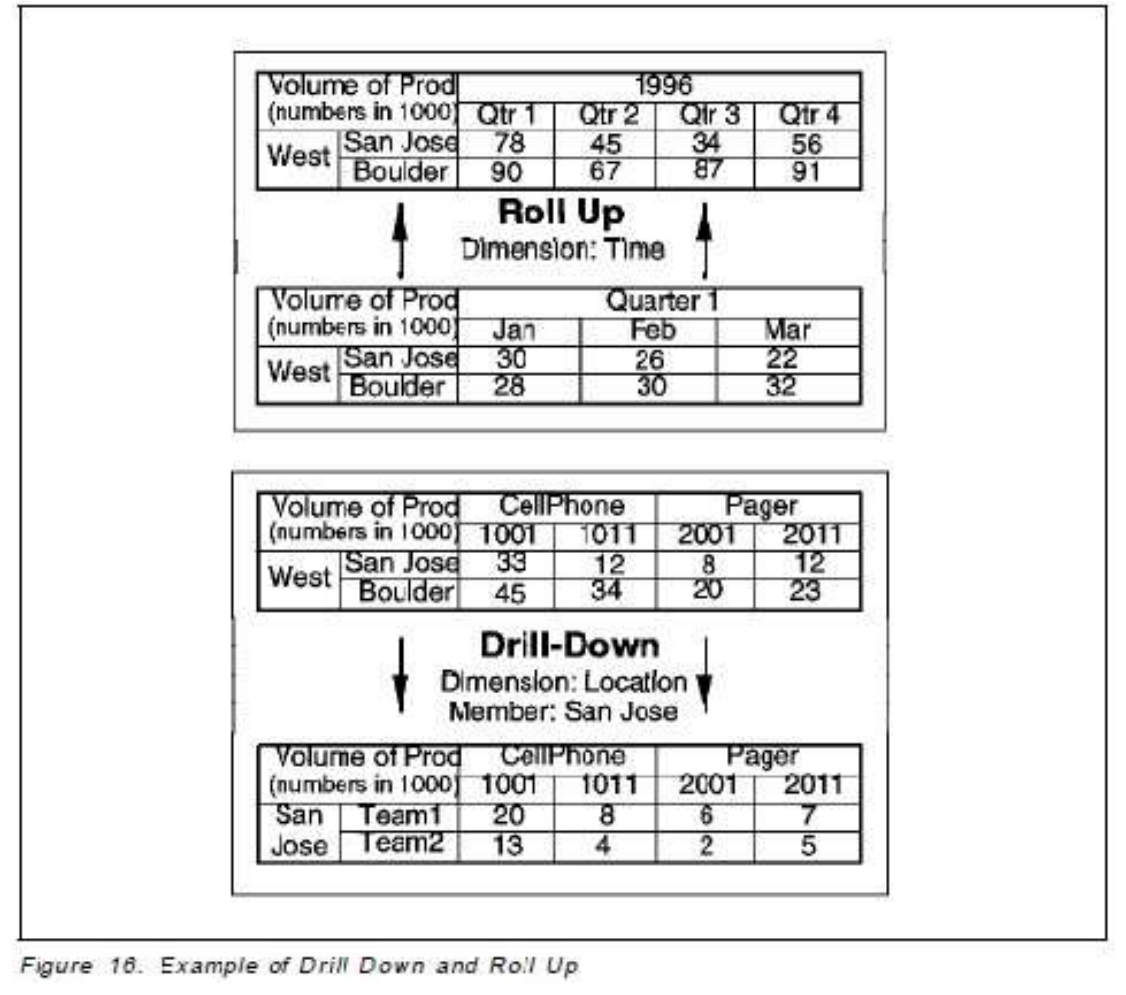
\includegraphics[width=\textwidth]{slide/rollup_drilldown.png}
    \caption{Roll-up và drill-down}
\end{subfigure}
\hfill
\begin{subfigure}[b]{0.56\textwidth}
    \centering
    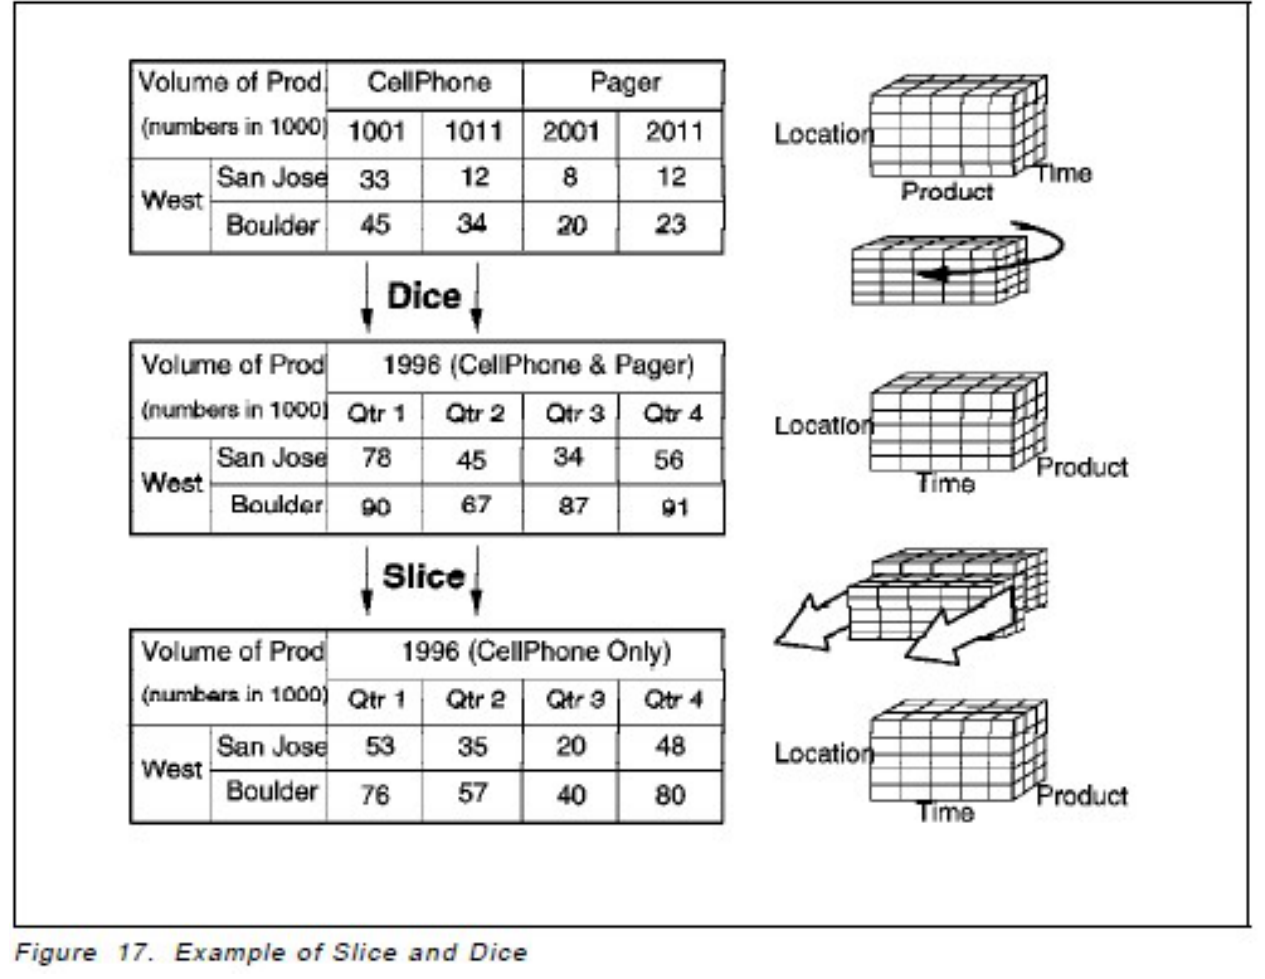
\includegraphics[width=\textwidth]{slide/slice_dice.png}
    \caption{Dice và slice}
\end{subfigure}
\caption{Các phép thao tác OLAP}
\label{fig:olap}
\end{figure}

\subsection{Hệ hỗ trợ ra quyết định}
\subsubsection{Định nghĩa và quá trình ra quyết định}
Bốn pha ra quyết định của Simon (Hình~\ref{fig:simon}) là khung mà Chương 6 dùng để xếp các màn hình của DSS: tìm hiểu (intelligence) phát hiện và phát biểu vấn đề, thiết kế (design) dựng mô hình với các biến và quan hệ giữa chúng, lựa chọn (choice) chọn một giải pháp từ mô hình, thực hiện (implementation) đưa giải pháp vào thực tế. Kết quả thực hiện được theo dõi và phản hồi về các pha trước. Hệ hỗ trợ ra quyết định (DSS), theo Turban và Aronson~\cite{turban2005}, là hệ thống thông tin giúp hỗ trợ và cải thiện việc ra quyết định.

\begin{figure}[!htbp]
\centering
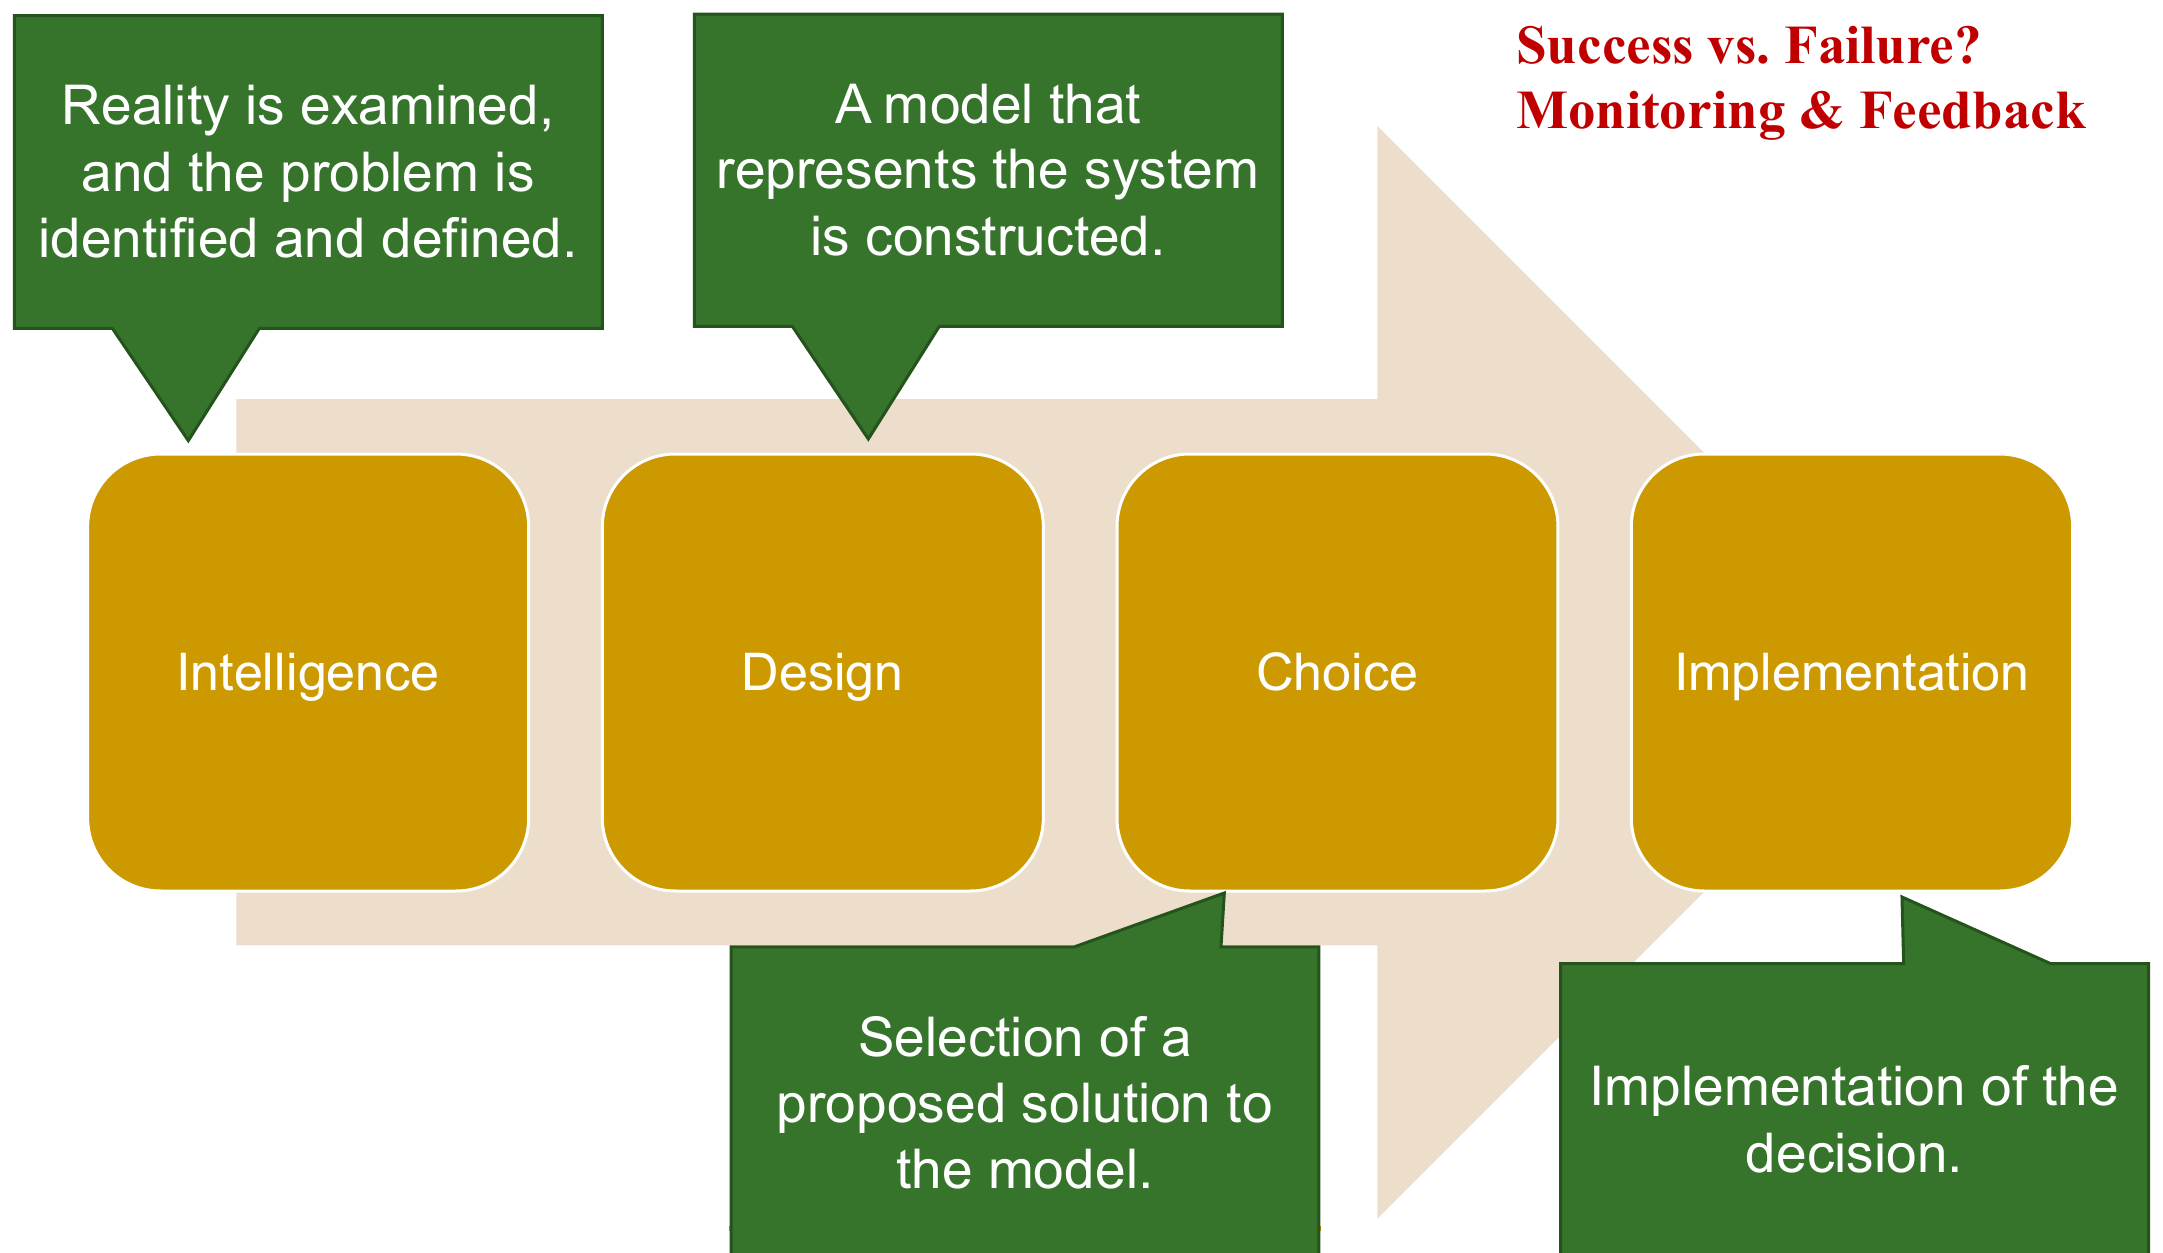
\includegraphics[width=0.72\textwidth]{slide/simon.png}
\caption{Bốn pha của quá trình ra quyết định theo Simon}
\label{fig:simon}
\end{figure}

\subsubsection{Đặc điểm và thành phần của DSS}
DSS hỗ trợ các vấn đề bán cấu trúc và phi cấu trúc cho nhà quản lý ở mọi cấp, nhắm tới hiệu quả của quyết định hơn là hiệu suất tính toán, và con người vẫn kiểm soát máy. Đó là ba trong 14 đặc điểm mà Turban và Aronson~\cite{turban2005} liệt kê (Hình~\ref{fig:dac_trung_dss}). Chương 6 nêu những đặc điểm trong số này mà hệ thống của đề tài đáp ứng đầy đủ.

\begin{figure}[!htbp]
\centering
% Vẽ lại từ hình trong slide (bản scan bị lỗi chữ): DSS ở giữa, bảy đặc điểm mỗi bên
\begin{tikzpicture}[
    dd/.style={draw=black!70, rounded corners=2pt, fill=white, align=left, text width=5.5cm, font=\footnotesize, inner sep=3pt, minimum height=9mm},
    day/.style={black!50, thin}]
    \foreach \i/\chu in {
        1/{(1) Vấn đề bán cấu trúc và phi cấu trúc},
        2/{(2) Hỗ trợ nhà quản lý ở mọi cấp},
        3/{(3) Hỗ trợ cá nhân và nhóm},
        4/{(4) Quyết định phụ thuộc nhau hoặc tuần tự},
        5/{(5) Hỗ trợ đủ bốn pha ra quyết định},
        6/{(6) Nhiều phong cách và quy trình ra quyết định},
        7/{(7) Thích nghi và linh hoạt}} {
        \node[dd, anchor=east] (t\i) at (-1.5, {-(\i-1)*1.0}) {\chu};
    }
    \foreach \i/\chu in {
        8/{(8) Tương tác, dễ sử dụng},
        9/{(9) Hiệu quả, không chỉ hiệu suất},
        10/{(10) Con người kiểm soát máy},
        11/{(11) Người dùng cuối dễ tự phát triển},
        12/{(12) Mô hình hoá và phân tích},
        13/{(13) Truy cập dữ liệu},
        14/{(14) Độc lập, tích hợp hoặc trên nền Web}} {
        \node[dd, anchor=west] (t\i) at (1.5, {-(\i-8)*1.0}) {\chu};
    }
    \node[draw, thick, rounded corners=3pt, fill=gray!15, minimum width=18mm, minimum height=10mm, font=\small\bfseries] (dss) at (0, -3.0) {DSS};
    \foreach \i in {1,...,7} \draw[day] (dss.west) -- (t\i.east);
    \foreach \i in {8,...,14} \draw[day] (dss.east) -- (t\i.west);
\end{tikzpicture}
\caption{Mười bốn đặc điểm của DSS}
\label{fig:dac_trung_dss}
\end{figure}

Bốn thành phần của một DSS (Hình~\ref{fig:thanh_phan_dss})~\cite{turban2005} cũng là bốn phân hệ của hệ thống ở Chương 6: quản lý dữ liệu (lấy dữ liệu từ kho hoặc nguồn khác), quản lý mô hình (lưu và chạy các mô hình thống kê, tài chính, khoa học quản lý), quản lý tri thức (quy tắc nghiệp vụ và tri thức chuyên gia) và giao diện người dùng.

\begin{figure}[!htbp]
\centering
\begin{tikzpicture}[
    tp/.style={draw=black!70, rounded corners=2pt, fill=white, minimum width=30mm, minimum height=10mm, align=center, font=\small},
    noi/.style={{Stealth[length=2mm]}-{Stealth[length=2mm]}, thick}]
    \node[tp] (data) {Quản lý dữ liệu};
    \node[tp, right=14mm of data] (model) {Quản lý mô hình};
    \node[tp, fill=gray!15, thick, below=8mm of $(data)!0.5!(model)$] (ui) {Giao diện người dùng};
    \node[tp, right=10mm of model, yshift=-9mm] (kb) {Quản lý tri thức};
    \node[tp, below=8mm of ui] (user) {Người ra quyết định};
    \draw[noi] (data) -- (model);
    \draw[noi] (data) -- (ui);
    \draw[noi] (model) -- (ui);
    \draw[noi] (kb) -- (ui);
    \draw[noi] (ui) -- (user);
    \node[tp, left=10mm of data] (src) {Kho dữ liệu,\\nguồn khác};
    \draw[-{Stealth[length=2.5mm]}, thick] (src) -- (data);
\end{tikzpicture}
\caption{Các thành phần của một DSS}
\label{fig:thanh_phan_dss}
\end{figure}

\subsubsection{Mô hình hoá và phân tích trong DSS}
Giá trị ròng $Z$ mà Chương 6 cực đại hoá là một biến kết quả theo cách phân loại của Turban và Aronson~\cite{turban2005}. Mô hình toán trong DSS có ba loại biến: biến quyết định là những gì người ra quyết định chọn được, biến không kiểm soát được (tham số) là yếu tố môi trường như giới hạn ngân sách, biến kết quả đo mức độ đạt mục tiêu. Bài toán phối hợp sản phẩm (product-mix) là ví dụ kinh điển: tìm số lượng từng sản phẩm để cực đại $Z$ trong giới hạn tài nguyên, giải bằng quy hoạch tuyến tính hoặc quy hoạch nguyên. Thay sản phẩm bằng khách hàng và tài nguyên bằng ngân sách chăm sóc, ta có bài toán ở Chương 6.

Quyết định diễn ra trong một trong ba điều kiện. Chắc chắn: biết chính xác kết quả của mỗi phương án. Rủi ro: mỗi phương án có nhiều kết quả và biết xác suất của từng kết quả, lúc đó chọn phương án có giá trị kỳ vọng lớn nhất:
\begin{equation}
    EV(a) = \sum_{k} P(s_k)\, v(a, s_k)
\end{equation}
với $P(s_k)$ là xác suất của tình huống $s_k$ và $v(a, s_k)$ là kết quả của phương án $a$ trong tình huống đó. Bất định: không ước lượng được xác suất, nên chọn theo cách lạc quan (maximax) hoặc bi quan (maximin). Chương 5 dùng điều kiện rủi ro với xác suất lấy từ mô hình, còn Chương 6 phải dùng cả ba cách khi tỷ lệ thành công của chăm sóc chưa đo được.

Có mô hình rồi, DSS cho người dùng xoay phương án theo bốn kiểu phân tích~\cite{turban2005}: what-if (đổi một giả định rồi xem kết quả), độ nhạy (đổi một biến nhiều lần để xem kết quả nhạy đến đâu), tìm mục tiêu (tìm đầu vào cần có để đạt một mục tiêu) và tối ưu hoá (tìm giá trị tốt nhất của biến mục tiêu). Chương 6 dùng cả bốn.

\subsection{Phương pháp khai phá dữ liệu}
Đề tài dùng ba bài toán khai phá dữ liệu: phân lớp để chấm điểm nguy cơ, gom cụm để chia nhóm khách, luật kết hợp để gợi ý sản phẩm. Khai phá dữ liệu là quá trình tìm mẫu và tri thức có ích từ dữ liệu lớn~\cite{han2011}, một bước trong quy trình khám phá tri thức (KDD) ở Hình~\ref{fig:kdd}: làm sạch và tích hợp, đưa vào kho, chọn và biến đổi, khai phá, đánh giá và trình bày. Chương 3 và 4 lo các bước trước khai phá, Chương 5 và 6 lo hai bước sau.

\begin{figure}[!htbp]
\centering
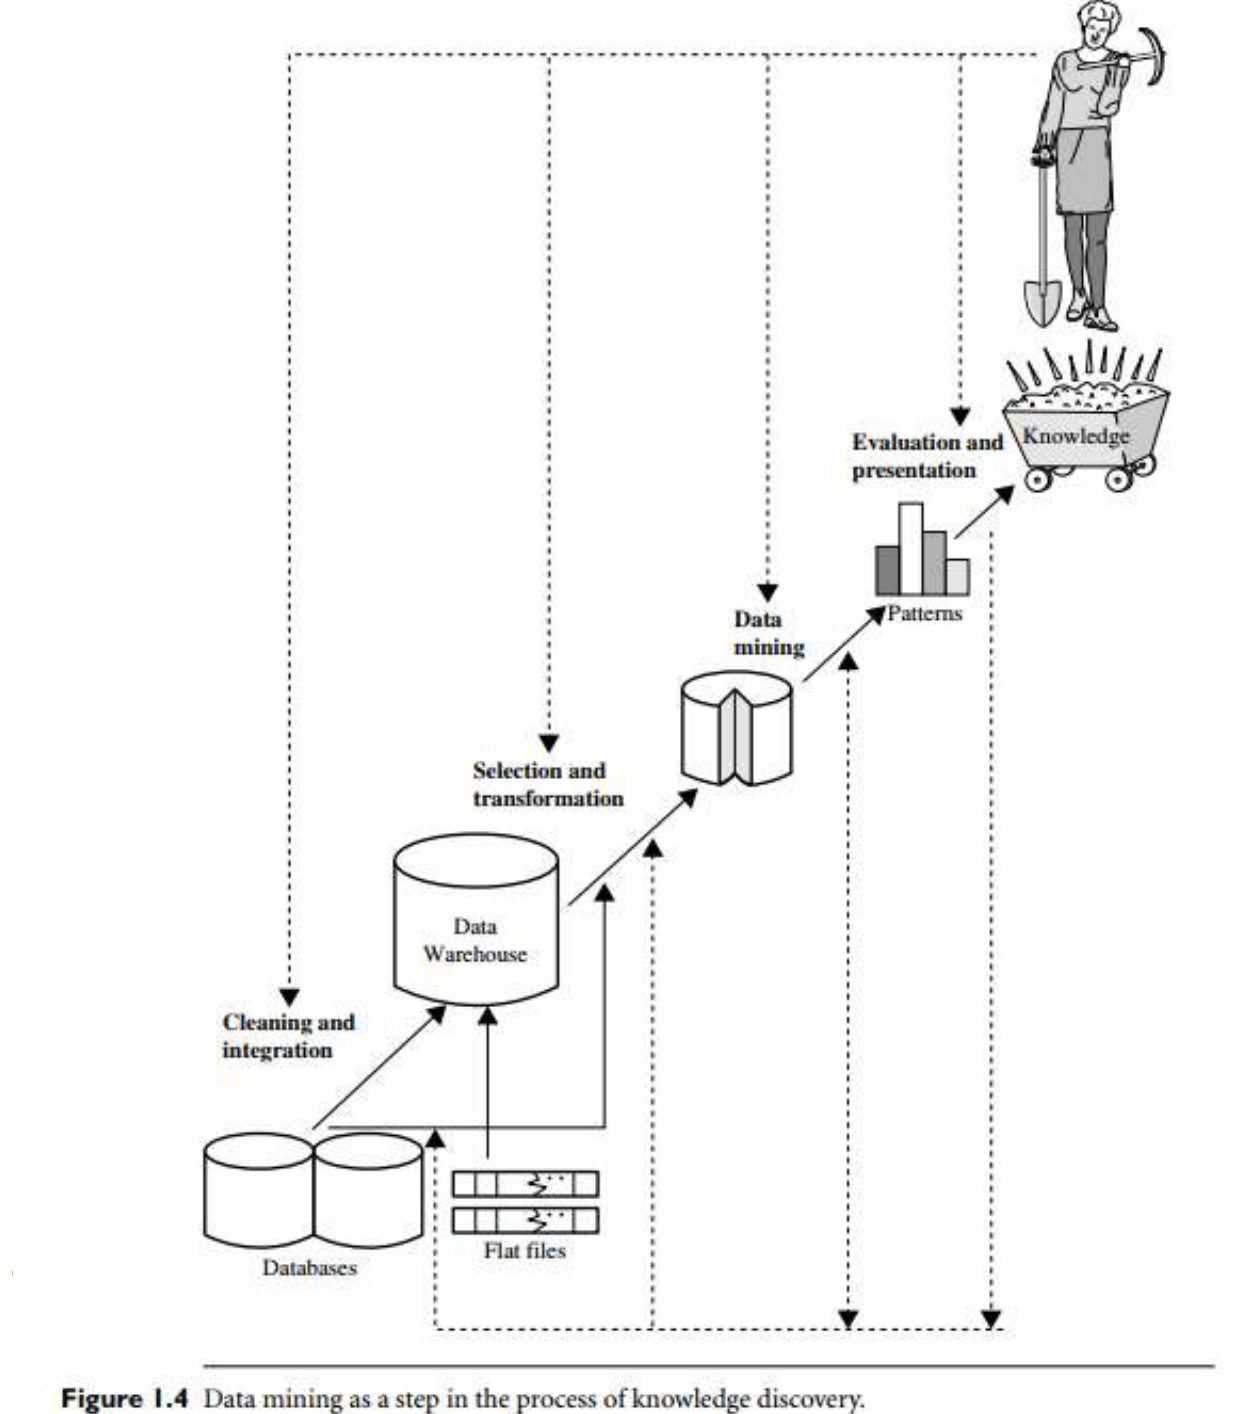
\includegraphics[width=0.4\textwidth]{slide/kdd.png}
\caption{Khai phá dữ liệu là một bước trong quy trình khám phá tri thức}
\label{fig:kdd}
\end{figure}

\subsubsection{Phân lớp và đánh giá mô hình}
Phân lớp (classification) đi qua hai bước~\cite{han2011}: bước học dựng mô hình từ tập huấn luyện đã có nhãn, bước phân lớp dùng mô hình đoán nhãn cho dữ liệu mới. Giữa hai bước, mô hình phải qua một tập thử có nhãn khác tập huấn luyện. Với hai lớp, kết quả thử gói trong ma trận nhầm lẫn (Bảng~\ref{tab:ma_tran_nham_lan}), từ đó ra sáu chỉ số~\cite{han2011}:
\begin{align}
    \text{Accuracy} &= \frac{TP + TN}{P + N}, &
    \text{Error rate} &= \frac{FP + FN}{P + N}, \\
    \text{Recall} &= \frac{TP}{P}, &
    \text{Specificity} &= \frac{TN}{N}, \\
    \text{Precision} &= \frac{TP}{TP + FP}, &
    F_1 &= \frac{2 \times \text{Precision} \times \text{Recall}}{\text{Precision} + \text{Recall}}.
\end{align}
Accuracy dễ bị đánh lừa khi một lớp chiếm đa số, đúng tình huống của đề tài vì phần lớn khách mang nhãn có nguy cơ (Chương 4). Khi đó precision, recall và specificity mới cho biết mô hình sai ở lớp nào.

\begin{table}[!htbp]
\centering
\caption{Ma trận nhầm lẫn cho bài toán hai lớp}
\label{tab:ma_tran_nham_lan}
\begin{tabular}{llcc}
\toprule
 & & \multicolumn{2}{c}{\textbf{Dự đoán}} \\
 & & Dương & Âm \\
\midrule
\multirow{2}{*}{\textbf{Thực tế}} & Dương ($P$) & TP & FN \\
 & Âm ($N$) & FP & TN \\
\bottomrule
\end{tabular}
\end{table}

\subsubsection{Chỉ số bổ sung và kiểm định theo thời gian}\label{sec:chisobosung}
Sáu chỉ số trên đều cần một ngưỡng để đổi xác suất thành nhãn. DSS của đề tài không dùng nhãn mà dùng thẳng xác suất để tính giá trị kỳ vọng, nên cần thêm bốn chỉ số đo chính xác suất, cả bốn đều ngoài nội dung môn học.
\begin{itemize}
    \item \textbf{ROC-AUC}~\cite{fawcett2006} là xác suất mô hình xếp một bản ghi lớp dương cao hơn một bản ghi lớp âm. Giá trị 0,5 là đoán ngẫu nhiên, 1 là xếp hạng hoàn hảo. Chỉ số này không phụ thuộc ngưỡng và tỷ lệ hai lớp.
    \item \textbf{Brier}~\cite{brier1950} là trung bình bình phương sai số giữa xác suất dự đoán và nhãn thật (0 hoặc 1), càng nhỏ càng tốt. Chỉ số này đo xác suất có sát thực tế hay không, điều ROC-AUC không đo được vì ROC-AUC chỉ xét thứ tự.
    \item \textbf{ECE} (sai số hiệu chỉnh kỳ vọng) chia bản ghi theo khoảng xác suất dự đoán rồi lấy trung bình có trọng số của chênh lệch giữa xác suất dự đoán và tỷ lệ lớp dương thật trong từng khoảng. Mô hình đoán 80\% thì trong nhóm đó thực tế phải có khoảng 80\% bản ghi lớp dương.
    \item \textbf{Lift theo decile} chia bản ghi thành mười phần bằng nhau theo điểm giảm dần, rồi so tỷ lệ lớp dương của từng phần với tỷ lệ chung. Lift của phần đầu càng cao thì danh sách ưu tiên càng đáng tin.
\end{itemize}
Dữ liệu của đề tài có thứ tự thời gian và mô hình phải đoán tương lai, nên tập học và tập thử chia theo thời gian, không chia ngẫu nhiên: học trên dữ liệu đến một mốc, thử trên dữ liệu sau mốc, lặp ở nhiều mốc. Chia ngẫu nhiên để thông tin tương lai lọt vào tập học và cho kết quả lạc quan hơn thật. Nhãn rời bỏ cũng phải suy từ cửa sổ quan sát: khách coi là rời bỏ nếu không giao dịch trong một khoảng cố định sau mốc, và một mốc chỉ dùng được khi cửa sổ của nó đã khép lại. Đó là lý do Chương 4 có 20 mốc nhưng chỉ 19 mốc có nhãn.

\subsubsection{Cây quyết định}
Chương 5 dùng cây quyết định làm mô hình đối chứng và lấy luật của lá để giải thích kết quả, vì mỗi đường đi từ gốc tới lá đọc được thành một luật IF--THEN mà người không chuyên tự kiểm tra được. Cây chia dữ liệu dần theo từng thuộc tính: mỗi nút trong kiểm tra một thuộc tính, mỗi nhánh là một kết quả kiểm tra, mỗi lá là một nhãn lớp. Các thuật toán phổ biến là ID3, C4.5 và CART~\cite{han2011}, khác nhau ở cách chọn thuộc tính chia tại mỗi nút. ID3 dùng độ lợi thông tin. CART, thuật toán đề tài dùng, chọn thuộc tính làm chỉ số Gini giảm nhiều nhất (công thức này ngoài nội dung môn học):
\begin{equation}
    Gini(D) = 1 - \sum_{i=1}^{m} p_i^2
\end{equation}
với $p_i$ là tỷ lệ bản ghi thuộc lớp $C_i$ trong tập $D$. Gini bằng 0 khi nút chỉ còn một lớp.

\subsubsection{Bộ phân lớp Naive Bayes}
Naive Bayes là mô hình chấm điểm chính của đề tài, một phần vì nó cho thẳng xác suất của từng lớp (Chương 5 nêu đủ lý do chọn). Mô hình dựa trên định lý Bayes~\cite{han2011}:
\begin{equation}
    P(C_i \mid X) = \frac{P(X \mid C_i)\, P(C_i)}{P(X)}
\end{equation}
với $X$ là một bản ghi và $C_i$ là một lớp. Mô hình gán $X$ vào lớp có $P(X \mid C_i)P(C_i)$ lớn nhất. Để tính $P(X \mid C_i)$ cho đơn giản, mô hình giả định các thuộc tính độc lập với nhau khi đã biết lớp:
\begin{equation}
    P(X \mid C_i) = \prod_{k=1}^{n} P(x_k \mid C_i)
\end{equation}
Giả định này hiếm khi đúng hẳn, nhưng mô hình vẫn thường xếp hạng tốt. Một giá trị thuộc tính chưa từng xuất hiện trong một lớp sẽ cho xác suất 0 và kéo cả tích về 0, nên người ta làm trơn Laplace bằng cách cộng một số nhỏ vào mỗi lần đếm (ngoài nội dung môn học).

\subsubsection{Mạng nơ-ron, gom cụm và luật kết hợp}
Ba kỹ thuật còn lại mỗi thứ phục vụ một việc. Mạng nơ-ron nhiều tầng (MLP) chỉ dùng để so sánh với Naive Bayes: gồm tầng đầu vào, một hay nhiều tầng ẩn và tầng đầu ra, huấn luyện bằng lan truyền ngược~\cite{han2011}, phần này ngoài nội dung môn học.

Gom cụm K-means chia khách thành các nhóm hành vi ở Chương 6. Thuật toán chia dữ liệu thành $k$ cụm~\cite{han2011}: chọn $k$ tâm ban đầu, gán mỗi điểm vào cụm có tâm gần nhất, cập nhật tâm bằng trung bình của cụm, lặp đến khi ổn định. Số cụm thường chọn bằng phương pháp khuỷu tay (elbow) trên tổng bình phương khoảng cách trong cụm, hoặc bằng hệ số Silhouette (đo mỗi điểm gần cụm của mình hơn cụm kế bên bao nhiêu, từ $-1$ đến 1, càng cao càng tốt).

Luật kết hợp, ví dụ bằng thuật toán Apriori, tìm các mặt hàng hay được mua cùng nhau để gợi ý sản phẩm. Luật $A \Rightarrow B$ đo bằng ba chỉ số:
\begin{equation}
    \text{support} = P(A \cup B), \qquad
    \text{confidence} = \frac{P(A \cup B)}{P(A)}, \qquad
    \text{lift} = \frac{P(A \cup B)}{P(A)\,P(B)}
\end{equation}
Lift lớn hơn 1 nghĩa là $A$ và $B$ đi cùng nhau nhiều hơn mức ngẫu nhiên.

\subsubsection{Đặc trưng RFM và phân hạng ABC}\label{sec:rfmabc}
Ba con số đi theo mỗi khách suốt báo cáo là RFM: Recency là số ngày từ lần mua gần nhất, Frequency là số lần mua, Monetary là tổng tiền đã mua. Chúng tính được từ riêng dữ liệu giao dịch, vừa làm đầu vào cho phân lớp và gom cụm, vừa đủ dễ đọc để người quản lý tự kiểm tra. Phân hạng ABC~\cite{flores1986} xếp các đối tượng theo giá trị giảm dần rồi chia hạng theo tỷ trọng giá trị tích luỹ, ví dụ hạng A gồm những đối tượng đầu tiên gộp lại chiếm 80\% tổng giá trị. Phương pháp này sinh ra để quản lý tồn kho, đề tài mượn sang xếp hạng khách theo Monetary.
